\clearpage
\section{Close proximity detection}

During the autonomous navigation the rover will be using 4 ultrasonic sensors for close proximity detection. These sensors will be placed at the same height as the wheels to help detect objects within a close distance of the rover.

\begin{figure}[H]
	\centering
	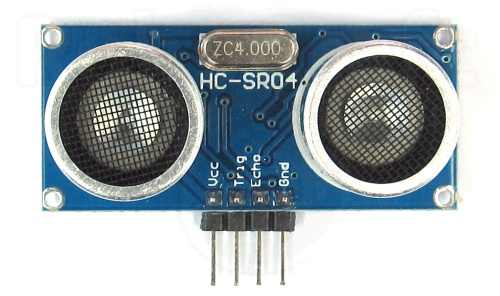
\includegraphics[width=.4\linewidth]{images/hcsr40.jpg}
	\caption{The specific ultrasonic sensors are 4 \textbf{HC-SR04}.}
	\label{fig:sub2}
\end{figure}

\iffalse

\begin{table}[H]
\centering
\begin{tabular}{|l|l|}
\hline
\textbf{Name}        & \textbf{HC-SR04 Ultrasonic Module} \\ \hline
Operating Voltage    & DC-5V                              \\ \hline
Operating Current    & 15mA                               \\ \hline
Operating Frequency  & 40KHZ                              \\ \hline
Range                & 2-400cm                            \\ \hline
Input trigger signal & 10us pulse                         \\ \hline
Measuring angle      & 15 degree                          \\ \hline
\end{tabular}
\caption{Information from the datasheet\cite{hcsr40datesheet}}
\end{table}

\fi

To use these specific ultrasonic sensors with the Raspberry Pi a voltage divider is needed. Since the sensor take 5V in, the out put will also be 5V. The Raspberry Pi's GPIO ports operate at 3.3V, so the voltage divider is used to limit the voltage going into the input port.
When the sensor are initially connected they require a few milliseconds to initialize, before they can be used to take measurements.

The trigger pin on the sensor is connect to a GPIO-OUT and the echo pin is connected to a GPIO-IN.

\begin{figure}[H]
	\centering
	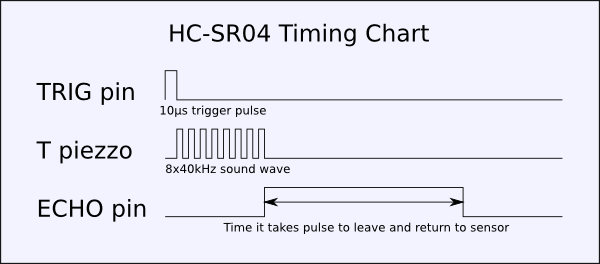
\includegraphics[width=.5\linewidth]{images/hcsr04timingchart.png}
	\caption{The HC-SR04 timing chart\cite{hcsr04timingchart}}
\end{figure}

A 10us pulse is sent from the sensor using the trigger pin, the echo pin receives a HIGH-pulse equivalent to how long it took to hear the echo. This means that length of this high-pulse is proportional to how far away the object is that distance is being measured between.\cite{ultrasonichowitworks}

$distance = \frac{(stoptime-startime) * 34000}{2}$

The above calculation is done using the speed of sound which is $speed = 340m/s$, which in centimetres is $34000cm/s$.